\documentclass[a4paper]{article}
\usepackage[pdftex]{graphicx}
\usepackage[utf8]{inputenc}
\usepackage{enumerate}
\usepackage{icomma}
\usepackage{siunitx}
\sisetup{locale=DE} 
\usepackage{amssymb}
\usepackage{eurosym}
\usepackage{tikz}
\usepackage{href-ul}
\hypersetup{
	colorlinks=true,
	linkcolor=blue,
	urlcolor=blue}
\usepackage{geometry}
\geometry{a4paper, top=15mm, left=15mm, right=15mm, bottom=15mm,
	headsep=10mm, footskip=12mm}

\begin{document}
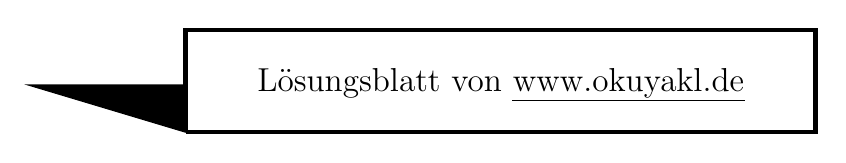
\begin{tikzpicture}(10,3)
	\draw[ultra thick](2,0) --(10,0) -- (10,1.3) --(2,1.3) -- (2,0);
	\draw[fill=black](2,0)-- (0,.6) -- (2,.6) -- (2,0);
	\node at (6,.6) {\large Lösungsblatt von \href{https://www.okuyakl.de}{www.okuyakl.de}};
\end{tikzpicture}
\vspace{0.5 cm}
\fbox{\begin{minipage}{0.45\textwidth}
	\noindent {\bf Aufgabe 1. a)}\\
	Geeignet ist hier das Additionsverfahren:
	$$
	\renewcommand{\arraystretch}{2}
	\begin{array}{rrcll}
	I.& -8x + 4y &=& 24 &|\cdot 5 \\
	II. & 17x-5y &=& -9 &|\cdot 4 \\
	\hline 
	I'.& -40x +20y &=& 120 \\
	II'.& 68x-20y &=& -36 \\
	\hline
	I'+II': & 28x &=& 84 &|:28 \\
	& x &=& 3 \\
	I. & -8\cdot 3 + 4y &=& 24 &| +24 \\
	& 4y &=& 48 &|:4 \\
	& y &=& 12
	\end{array}
	$$ 
\end{minipage}}
\hfill
\fbox{\begin{minipage}{0.45\textwidth}
	\noindent {\bf Aufgabe 1. b)}\\
	Hier ist auch das Additionsverfahren am geeignetsten:
	$$
	\renewcommand{\arraystretch}{2}
	\begin{array}{rrcll}
	I. & 6x -12y &=& -6 \\
	II.& -6x+4y &=&-14 \\
	\hline
	I+II: & -8y &=& -20 &|:(-8)\\
	& y &=& 2,5 \\
	I.& 6x -30 &=& -6 &|+30\\
	& 6x &=& 24 &|:6 \\
	& x &=& 4 
	\end{array}
	$$
\end{minipage}}
	
\fbox{ 
\begin{minipage}{0.45\textwidth}
	\noindent {\bf Aufgabe 2. a)}\\
	Schenkellänge $x$, Basislänge $y$:
	$$
	\renewcommand{\arraystretch}{2}
	\begin{array}{rrcll}
	I & 2x +y &=& 20 \\
	II & y &=& x+2 &| -x \quad |\cdot (-1)\\
	 & x-y &=& -2 \\
	\hline 
	I+II:& 3x &=& 18 &|:3\\
	& x&=& 6 \\
	II & y &=& 6+2 &=8
	\end{array}
	$$
\end{minipage}}
\hfill
\fbox{ 
\begin{minipage}{0.45\textwidth}
	\noindent {\bf Aufgabe 2. b)}\\
Rechnung Nr. 1 $x$; Rechnung Nr. 2 $y$:
$$
\renewcommand{\arraystretch}{2}
\begin{array}{rrcll}
I. & 0,02x +0,03y &=& 144 &|\cdot 50\\
II. & 0,025x + 0,025y &=& 140 &|\cdot(-40)\\
\hline
I'& x + 1,5y &=& 7200 \\
II'&-x -y &=& -5600 \\
\hline
I'+II'& 0,5y &=& 1600 \\
& y &=& 3200 \\
I'& x+1,5\cdot 3200&=& 7200 &|-4800\\
 & x &=& 2400 
\end{array}
$$
\end{minipage}}

\fbox{
	\begin{minipage}{0.45\textwidth}
	\noindent {\bf Aufgabe 2. c)}\\
	Menge Orangennektar  $x$; Menge Apfelsaft $y$: Fruchtgehalt Bowle $0,5$
	$$
	\renewcommand{\arraystretch}{2}
	\begin{array}{rrcll}
	I & x + y &=& 3 &|\cdot (-0,3)\\
	I'& -0,3x -0,3y &=& -0,9 \\
	II & 0,3x + 0,8y &=& 3\cdot 0,5 \\
	\hline
	I'+II& 0,5y &=& 0,6 &|:0,5\\
	 & y &=& 1,2\\
	I & x +1,2 &=& 3 &|-1,2\\
	& x &=& 1,8
	\end{array}
	$$ 
\end{minipage}}
\hfill
\fbox{
\begin{minipage}{0.45\textwidth}
	\noindent{\bf Aufgabe 3. a)}\\
	Wir beseitigen alle Brüche, indem wir beide Gleichungen mit 6 mulitplizieren und nach x und y sortieren. Anschließend multiplizieren wir wie folgt und addieren:
	$$
	\renewcommand{\arraystretch}{2}
	\begin{array}{rrcll} 
	I & 2 x + y &=& -12 &|\cdot (-4) \\
	II &  -3x + 4y &=&-48 \\
	\hline
	I+II & -11x &=& 0 & \\
	& x   &=& 0 \\
	\textnormal{in I:} & y &=& -12 \\
	\hline 
	\end{array}  
	$$    
\end{minipage}}

\fbox{
\begin{minipage}{0.4\textwidth}
	\noindent{\bf Aufgabe 3. b)}\\
	$$\renewcommand{\arraystretch}{2}D_x = \left| \begin{array}{cc} 14 & 3 \\
	1 & 3,5 \end{array}\right| = 46$$
	$$\renewcommand{\arraystretch}{2}D_y = \left| \begin{array}{cc} -2 & 14 \\
	1,5 & 1 \end{array}\right| = -23$$
	$$\renewcommand{\arraystretch}{2}D = \left| \begin{array}{cc} -2 & 3 \\
	1,5 & 3,5 \end{array}\right| = -11,5$$
	$$x={D_x\over D}= -4 \qquad y={D_y\over D}=2$$
\end{minipage}}
\hfil
\fbox{
	\begin{minipage}{0.4\textwidth}
		\noindent{\bf Aufgabe 4.}\\
		Die Formel für die Parallelogrammfläche ist 
		$$I:\qquad A=a \cdot h=\SI{12}{\centi\meter}^2$$ 
		Weiter gilt: $$II:\quad 2a + 2b =\SI{18}{\centi\meter}$$ 
		$$III: \quad 2b=a$$ 
		$$III \quad \textnormal{in}\quad II: \quad 2a + a =18$$
		$$ \Rightarrow \quad a=\SI{6}{\centi\meter} \Rightarrow b=\SI{3}{\centi\meter} $$
		$$\textnormal{in I:}\quad 12 = 6 \cdot h \Rightarrow h=\SI{2}{\centi\meter}$$
	\end{minipage}}





\fbox{ 
	\begin{minipage}{0.45\textwidth}
		\noindent{\bf Aufgabe 5.}\\
		Es sei x die Menge an Kakaopulver und y die Menge an Kaffeepulver. Dann gilt:
		$$
		\renewcommand{\arraystretch}{2}
		\begin{array}{rrcl}
		I & x+y &=& 10 \\
		II & 5x + 8y &=& 68 \\
		\hline
		I \quad \textnormal{in} \quad II:& 5( 10-y) + 8y &=& 68 \\
		& 50 +3y &=& 68 \\
		& 3y &=& 18 \\
		& y &=& 6 \\
		& x &=& 4
		\end{array}
		$$
		Es werden 4 kg Kakaopulver und 6 kg Kaffeepulver verwendet.
	\end{minipage}}
	\hfill
	\fbox{ 
\begin{minipage}{0.45\textwidth}
	\noindent {\bf Aufgabe 6.}\\
	Rechteckseiten $x, y$:
	$$
	\renewcommand{\arraystretch}{2}
	\begin{array}{rrcll}
	I & 2x + 2y &=& 28 & |:2\\
	I'& x +y  &=& 14 \\
	II &(x+2)(y-1)&=& xy + 8 \\
	 & xy +2y - x-2 &=& xy +8 \\
	II'& -x+2y &=& 10 \\
	\hline
	I'+II'& 3y &=& 24 &|:3\\
	& y &=& 8 \\
	I'& x &=& 6 
	\end{array}
	$$ 	
\end{minipage}}

\fbox{ 
\begin{minipage}{0.45\textwidth}
\noindent {\bf Aufgabe 7.}\\
Schenkellänge $x$; Basislänge $y$:
$$
\renewcommand{\arraystretch}{2}
\begin{array}{rrcll}
I & 2x + y &=& 26 \\
II & x &=& {5\over 3}y \\
\hline
II~\textnormal{in}~I:& {10 \over 3}y + y &=& 26 \\
& {13 \over 3} y &=& 26 &|\cdot{3\over 13}\\
& y &=& 6 \\
II & x &=& 10
\end{array}
$$
\end{minipage}}
\hfill
\fbox{ 
\begin{minipage}{0.45\textwidth}
\noindent {\bf Aufgabe 8.}\\
Grundseite 1 $x$; Grundseite 2 $y$:
$$
\renewcommand{\arraystretch}{1.5}
\begin{array}{rrcll}
I & x-y &=& 4 &|\cdot 1,5\\
I'&1,5x-1,5y&=& 6 \\
II & 0,5\cdot(x+y)\cdot 3 &=& 21 \\
II'& 1,5x + 1,5 y &=& 21 \\
\hline
I'+II'& 3x &=& 27 \\
      &  x &=& 9 \\ 
I & 9-y &=& 4 \\ 
 & y &=& 5 
\end{array}
$$
\end{minipage}}
\vspace{0.5 cm}

	\noindent {\bf Aufgabe 8.}
	Wir legen fest: $x=$ Einerziffer $y=$ Zehnerziffer. Dann ist die Zahl $10y + x$, ihre Quersumme 
	$x+y$, und wir erhalten zwei Gleichungen:
	$$
	\renewcommand{\arraystretch}{1.5}
	\begin{array}{rcll}
	10y + x &=& 3 \cdot (x + y) +22 & (I)  \\ 
	y-1 &=& x                   & (II) \\
	
	\end{array}
	$$
	
	(I) lässt sich vereinfachen zu:
	$$ 7y - 2x = 22 \qquad (I')$$
	(II) setzen wir in (I') ein und erhalten:
	$$
	\renewcommand{\arraystretch}{1.5}
	\begin{array}{rcll}
	7y - 2(y-1) &=& 22   &   \\ 
	5y + 2 &=& 22   & |-2 \quad |:5\\
	y  &=& 4  &
	\end{array}
	$$
	Dieses Ergebnis setzen wir wieder in (II) ein, damit ist $x=3$. Die gesuchte Zahl ist also die 43.

\noindent \fbox{
\begin{minipage}{0.5\textwidth}
\noindent {\bf Aufgabe 9.}\\
$$\alpha + \beta = 180^\circ \quad \land \quad \alpha = \beta +30^\circ \quad \Rightarrow 2 \beta + 30^\circ =180^\circ $$
$$\Rightarrow \beta = 75^\circ \quad \alpha = 105^\circ $$ 	
\end{minipage}}
\hfill
\begin{minipage}{0.5\textwidth}
\begin{center}
	\includegraphics[width=7 cm]{../../viecher/endcomic.pdf}
	
	Hier geht es zurück zum \href{https://www.okuyakl.de/math/m9lgsL043/aa043.pdf}{Aufgabenblatt}
\end{center}

\end{minipage}



\end{document}

